

\chapter*{Chapter 2}
\section*{Jenis Variabel pada Python}
\par

 
Python memiliki seperangkat aturan pembuatan dan penulisan variabel yang jika dibandingkan dengan bahasa pemrograman lain seperti PHP, tidak jauh berbeda. Perlu diketahui bahwa Python merupakan bahasa pemrograman case sensitive. dan juga perlu diketahui nama variabel tidak boleh sama dengan salah satu nama yang masuk ke dalam kelompok {\textit{reserved word python}} , seperti : and, assert, break, class, continue, def, del, elif dsb. Variabel dalam python ada dua jenis yaitu variabel lokal dan global. berikut contoh variabel lokal dan global.

\begin{enumerate}
	\item buka Spyder lalu ketik kode berikut
	\begin{figure} [h]
	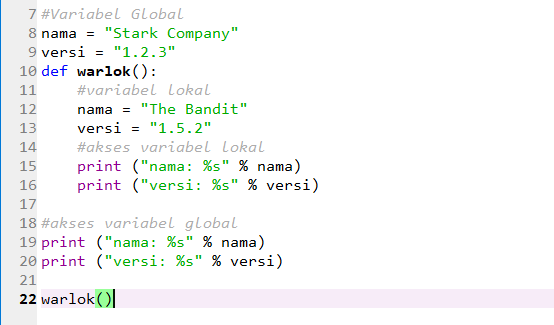
\includegraphics[width=9cm]{variabel/var1.png}
	\centering
	\end{figure}
	

	\item maka akan menghasilkan output seperti berikut
	\begin{figure} [h]
	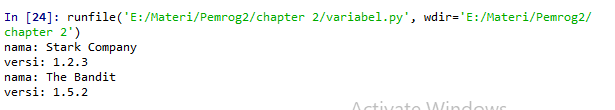
\includegraphics[width=12cm]{variabel/var2.png}
	\centering
	\end{figure}
	
	
\end{enumerate}